\subsection{Lesiones y patologías del sistema nervioso central}

El \acrfull{cns}, encargado de la planificación, iniciación y modulación del movimiento, comprende estructuras como la corteza cerebral, el tronco encefálico, el cerebelo y la médula espinal. A través de estas estructuras, el \acrshort{cns} procesa la información sensorial y genera impulsos nerviosos que son transmitidos a los músculos para producir movimiento \cite{emos_NeuroanatomyUpper2026}.

Las lesiones o patologías que afectan al \acrshort{cns} pueden dañar tanto las neuronas como las vías de comunicación entre ellas, alterando la transmisión de señales motoras y sensitivas. Como consecuencia, pueden aparecer deficiencias motoras, pérdida de sensibilidad, alteraciones del equilibrio o dificultades en la coordinación del movimiento \cite{emos_NeuroanatomyUpper2026}.

Entre las lesiones más relevantes se encuentran las \acrfull{scis}, producidas por causas traumáticas o no traumáticas que dañan parcial o totalmente la médula espinal. Este daño interrumpe la transmisión de señales nerviosas entre el cerebro y las regiones corporales situadas por debajo de la lesión. Los síntomas dependen tanto de la localización como de la gravedad del daño. Las lesiones cervicales pueden provocar tetraplegia, mientras que lesiones en regiones más bajas suelen derivar en paraplegia \cite{margetis_SpinalCord2026,ninds_SpinalCord}.

En la figura \ref{fig:spinal_cord} se puede ver un esquema de las lesiones medulares en función del area de lesión.

\begin{figure}[htbp]
    \centering
    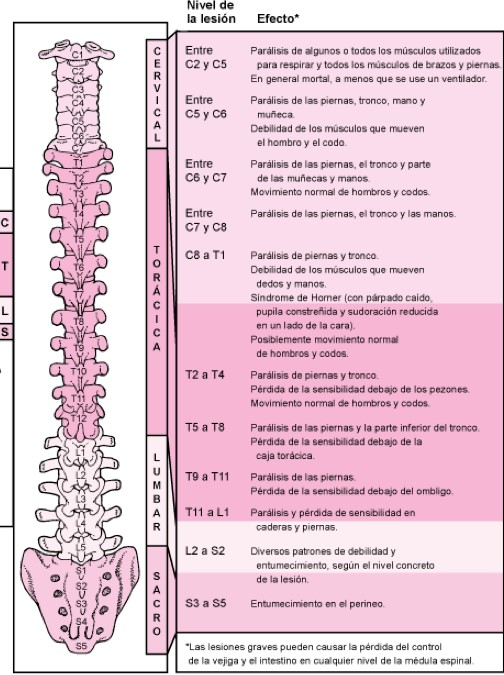
\includegraphics[width=0.80\textwidth]{img/spinal_cord_injury.png}
    %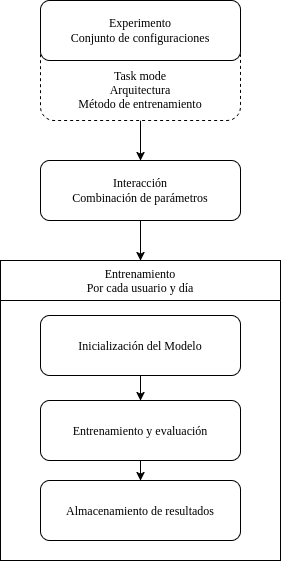
\includegraphics[height=\dimexpr\pagegoal-\pagetotal-\baselineskip\relax,width=\textwidth,keepaspectratio]{img/diagrama_pipeline.drawio.png}
    \caption{Esquema de las lesiones medulares en función del area de lesión \cite{corrallopez_TraumatismoMedular2023}}
    \label{fig:spinal_cord}
\end{figure}

Otra de las principales patologías del \acrshort{cns} son los accidentes cerebrovasculares o ictus. Estos pueden clasificarse en hemorrágicos, cuando se produce la rotura de un vaso sanguíneo cerebral, o isquémicos, cuando una obstrucción reduce o bloquea el flujo sanguíneo. En ambos casos se produce daño neuronal debido a la falta de oxígeno y nutrientes en el tejido cerebral afectado \cite{murphy_StrokeCauses2020}. Los ictus representan una de las principales causas de discapacidad motora adquirida y mortalidad a nivel mundial \cite{gao_RestoringCentral2022, emos_NeuroanatomyUpper2026, murphy_StrokeCauses2020}.

A pesar de la gravedad de estas lesiones, existe un potencial de rehabilitación en la neuroplasticidad. La neuroplasticidad la capacidad del \acrshort{cns} para modificar su estructura y funcionamiento, así como crear nuevas conexiones neuronales en respuesta a estímulos externos o internos \cite{emos_NeuroanatomyUpper2026,puderbaugh_Neuroplasticity2026}. La rehabilitación neurológica busca potenciar esta reorganización funcional de las áreas cerebrales no afectadas\cite{dipalma_FrontiersNeurorehabilitation2025}, creando nuevas conexiones mediante la repetición de tareas.

La rehabilitación constituye un proceso complejo que requiere un enfoque multidisciplinar y tratamientos personalizados. Aunque parte de la recuperación motora suele producirse durante los primeros meses tras la lesión, muchos pacientes continúan presentando secuelas permanentes en fases crónicas \cite{gao_RestoringCentral2022}. En estos casos, las tecnologías de asistencia, incluyendo los sistemas basados en interfaces cerebro-computadora (\acrshort{bci}), representan una herramienta prometedora para mejorar la autonomía y la interacción con el entorno.
